
%================1.1
\section{Giới thiệu}

%================1.1.1
\subsection{Giới thiệu việc học thống kê}

\textbf{Lịch sử ngắn gọn của việc học thống kê}

\hspace*{0.5cm}Thuật ngữ "Việc học thống kê" là khá mới (1980). Tuy nhiên nhiều mô hình khái niệm về nền tảng và mô hình toán học cho lĩnh vực này đã được phát triển từ lâu:
\begin{itemize} [label=--]
	\item Vào những năm 1800, Adrien-Marie Legendre và C.F. Gauss đã công bố các bài báo về phương pháp "bình phương tối thiểu" (Least-Squares Method - LS). Lý thuyết bình phương tối thiểu gắn với mô hình hồi quy tuyến tính là một trong các mô hình toán học được sử dụng phổ biến ở nhiều lĩnh vực khoa học khác nhau từ thiên văn học, hóa học, sinh học tiến hóa đến khoa học xã hội,...
	\item R.A. Fisher (1936) đề xuất phương pháp Phân tích tách biệt tuyến tính (Linear Discriminant Analysis - LDA) để dự đoán các biến đáp ứng định tính.
	\item Các nhà nghiên cứu đã đưa ra một hướng tiếp cận thay thế gọi là hồi quy Logistic (1940s).
	\item Đầu những năm 1970s, J.A. Nelder và R.W.M. Wedderburn đã đặt ra thuật ngữ các mô hình tuyến tính tổng quát hóa (Generalized Linear Models - GLM) cho toàn bộ lớp các phương pháp học thống kê bao gồm cả hồi quy tuyến tính, hồi quy logistic và các trường hợp đặc biệt (Hồi quy Poisson, Hồi quy Dirichlet).
	\item 1980, công nghệ máy tính được cải thiện đáng kể để các phương pháp phi tuyến có thể tính toán được (tính xấp xỉ) nhờ các công trình của Leo Breiman, Jerome H. Friedman, Richard A. Olshen, Charles J. Stone,... (giữa 1980s) họ đã giới thiệu và phát triển các mô hình cho sự phân lớp cây hồi quy (cây Bayes).
\end{itemize}
\hspace*{0.5cm}Các phương pháp học thống kê được phân thành hai loại chính và được mô tả trong sơ đồ sau
\begin{figure}[H]
	\centering
	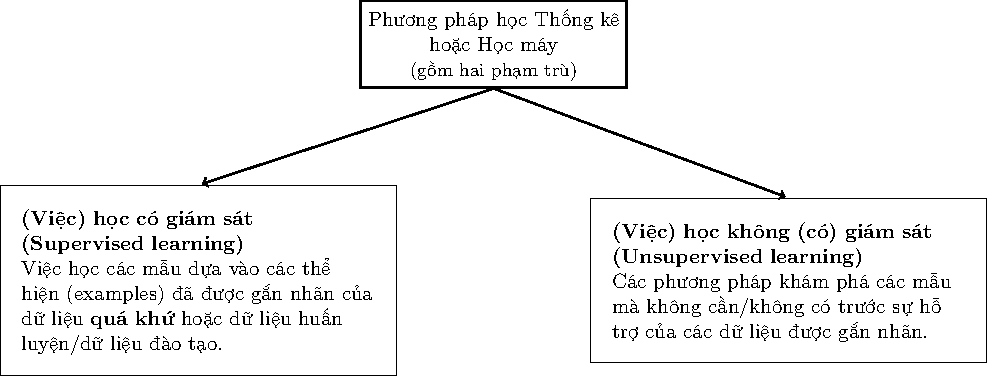
\includegraphics[width=0.85\textwidth]{image/phan_loai_hoc_may.pdf}

	% Thêm chú thích tên hình ở đây (để normal, không in nghiêng)
	\caption{Sơ đồ phân loại các phương pháp học thống kê.}
	\label{fig:phan_loai_hoc_may}
\end{figure}

%================1.1.2
\subsection{Tổng quan về việc học có giám sát}

Các phương pháp học có giám sát có các thành phần chung là:
\begin{itemize} [label=--]
	\item Tập biến đầu vào (Input variables): các thuật ngữ hiện đại được sử dụng trong lĩnh vực học máy (Machine Learning - ML)| Các đặc trưng (features) trong thống kê.
	\item Tập biến đầu ra (Output variables): được tính toán dựa vào quy luật đặt trên tập biến đầu vào. Các biến đầu ra còn được gọi là biến đáp ứng (responses).
\end{itemize}
Một số phương pháp thuộc phạm trù học có giám sát: Hồi quy logistic, Hồi quy tuyến tính,  K-NN (K lân cận gần nhất | K-Nearest Neighbors), LDA (Linear Discriminant Analysis), SVM (Support Vector Machine),...

Một số ứng dụng của phương pháp học có giám sát: 
\begin{itemize} [label=--]
	\item Dự đoán dựa trên hồ sơ nhân khẩu học, chế độ ăn uống, dữ liệu lâm sàng trước đó về khả năng một người có thể mắc bệnh tim (Phạm trù y sinh).
	\item Dự đoán giá một số loại cổ phiếu trong khoảng \textit{t} tháng từ thời điểm hiện tại dựa vào các số đo hiệu suất hoạt động của công ty và dữ liệu kinh tế liên quan (Phạm trù thị trường chứng khoán, cổ phiếu).
	\item Nhận dạng mẫu, chẳng hạn: nhận dạng chữ số, trong một mã nén (zipcode), chữ viết tay từ một ảnh số (Phạm trù chữ ký số, thương mại điện tử).  
\end{itemize}
Ta xét bài toán học theo quan điểm là bài toán tìm mối quan hệ | sự phụ thuộc mong muốn bằng việc sử dụng một tập hữu hạn các đối tượng quan sát (|dữ liệu được quan sát)
\begin{figure}[H]
	\centering
	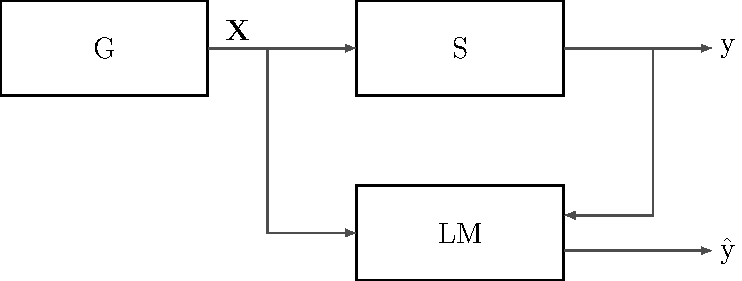
\includegraphics{image/mo_hinh_hoc_may.pdf}
	
	% Thêm chú thích tên hình ở đây (để normal, không in nghiêng)
	\caption{Mô hình toán học máy học.}
	\label{fig:mo_hinh_hoc_may}
\end{figure}
Mô hình chung của việc học từ ví dụ được mô tả ở hình trên như sau:
\begin{enumerate}
	\item[$(i)$] \textbf{Bộ sinh các giá trị của vectơ ngẫu nhiên} $(G)$ (\textit{Generator}): $\bm{x} \in \mathbb{R}^d$ được lấy (một cách) độc lập từ một hàm phân phối xác suất cố định nhưng không biết $F(\bm{x})$.
	\item[$(ii)$] \textbf{Bộ ( | người) giám sát} $(S)$ (\textit{Supervisor}): (mà) trả một giá trị ra (output) $y$ cho mỗi (vectơ) giá trị vào (input) $\bm{x}$, theo một phân phối điều kiện $F(y|\bm{x})$ cũng cố định nhưng không biết.
	\item[$(iii)$] \textbf{Một máy học} $(LM)$ (\textit{learning machine}) có khả năng thực hiện | thực thi tập các hàm $\{f(\bm{x}, \alpha)\}_{\alpha \in \Lambda}$, ở đây $\Lambda$ là một tập các tham số.
\end{enumerate}
Bài toán học là việc chọn, từ tập hợp các hàm $f(\bm{x}, \alpha)$ ($\alpha \in \Lambda$) đã cho, một hàm xấp xỉ tốt nhất cho đáp ứng của (bộ) giám sát. Sự lựa chọn hàm mong muốn là dựa trên một tập dữ liệu huấn luyện gồm $n$ quan sát được lấy một cách độc lập và chung phân phối (i.i.d. -- independent and identically distributed) $F(\bm{x},y) = F(\bm{x}) \cdot F(y|\bm{x})$
\begin{equation}
	(\bm{x}_1, y_1), (\bm{x}_2, y_2), \dots, (\bm{x}_n, y_n).
	\label{eq:1.1}
\end{equation}
Trong suốt quá trình, máy học theo dõi ``kiểu'' mẫu từ các cặp $(\bm{x}, y)$ (tập dữ liệu huấn luyện | tập dữ liệu đào tạo - \textit{the training set}). Sau quá trình đào tạo, máy phải trả về được giá trị $\hat{y}$ cho bất kỳ giá trị vào $\bm{x}$. Mục tiêu là giá trị $\hat{y}$ trả về ``gần'' (| xấp xỉ) với giá trị đáp ứng $y$ của bộ giám sát.

Mức độ tổn thất | mức độ chênh lệch giữa đáp ứng $y$ của bộ giám sát và đáp ứng $f(\bm{x}, \alpha)$ được cung cấp bởi máy học tương ứng với một giá trị vào $\bm{x}$ được ký hiệu là $L(y, f(\bm{x}, \alpha))$. Hàm $L(y, f(\bm{x}, \alpha))$ được gọi là \textbf{hàm tổn thất} (\textit{the loss functional}).

Khi đó, hàm rủi ro (the risk function), ký hiệu $R(\alpha)$, chính là tổn thất trung bình xác định bởi
\begin{equation}
	R(\alpha) = E[L(Y, f(X, \alpha))] = \int L(y, f(\bm{x}, \alpha)) dF(\bm{x}, y).
\end{equation}

$\rightarrow$ \textit{\textbf{Mục đích:}} Tìm hàm $f(\bm{x}, \alpha_0)$ ($\alpha_0 \in \Lambda$) mà cực tiểu $R(\alpha)$ (trên lớp hàm $\{f(\bm{x}, \alpha)\}_{\alpha \in \Lambda}$) trong ngữ cảnh: ta không biết hàm phân phối đồng thời $F(\bm{x}, y)$ và chỉ có sẵn thông tin mẫu được lấy từ nó (tập dữ liệu huấn luyện (\ref{eq:1.1})).

%=============1.1.3

\subsection{Bài toán phân loại mẫu}

% \subsubsection{Khái niệm về mẫu và nhận dạng mẫu thống kê}
Trong thống kê nhiều chiều, bài toán phân loại mẫu thống kê nhằm xác định một đối tượng quan sát thuộc về lớp hay quần thể nào dựa trên các đặc trưng đo được của nó. Giả sử có tập dữ liệu
\begin{equation*}
	\bm{x} = \{\bm{x}_1, \bm{x}_2, \dots, \bm{x}_n\}
\end{equation*}
Trong đó mỗi mẫu $\bm{x}_i$ được biểu diễn bởi $M$ biến đặc trưng. Tập dữ liệu được chia thành $k$ lớp
\begin{equation*}
	\bm{x} = \{C_1, C_2, \dots, C_k\}
\end{equation*}
với $C_j$ là lớp thứ $j$, $n_j$ là số mẫu thuộc lớp đó và
\begin{equation*}
	N=\sum_{j=1}^{k}n_j.
\end{equation*}
\hspace*{0.5cm}Mục tiêu của bài toán phân loại là xây dựng một quy tắc quyết định để khi có một mẫu mới, ta có thể gán mẫu đó vào lớp phù hợp nhất. Trong bối cảnh học có giám sát, nhãn lớp của các mẫu huấn luyện đã biết trước, nhờ đó có thể khai thác thông tin về cấu trúc giữa các lớp để xây dựng bộ phân loại. Đây là một phương pháp giảm chiều có giám sát, trong đó nhãn lớp được sử dụng để tìm ra không gian biểu diễn mới giúp tăng khả năng tách biệt giữa các lớp.
\begin{itemize}
	\item \textbf{Mẫu (Pattern):} Đứng ở góc độ toán học, một ``mẫu'' được biểu diễn như một vectơ đặc trưng $\mathbf{X} = \bm{x} \in \mathbb{R}^d$, đại diện cho các thuộc tính định lượng được trích xuất từ một đối tượng quan sát.
	
	\item \textbf{Nhận dạng (Recognition):} Là quá trình ánh xạ một mẫu $\bm{x}$ vào một trong các lớp (class) $\mathbf{y}$ thuộc một tập hợp rời rạc cho trước. Trong ngôn ngữ học máy, đây chính là bài toán Phân loại (Classification).
	
	\item \textbf{Nhận dạng mẫu thống kê (Statistical Pattern Recognition):} Phương pháp này xem xét sự biến thiên của các mẫu là ngẫu nhiên và giải quyết bài toán nhận dạng bằng cách tìm mối quan hệ bản chất giữa không gian đặc trưng $\mathcal{X}$ và không gian nhãn $\mathcal{Y}$ thông qua lý thuyết xác suất.
\end{itemize}
\hspace*{0.5cm}Đối với bài toán phân loại mẫu thống kê bằng hồi quy tuyến tính và hồi quy logistic, tư tưởng cốt lõi là xây dựng các hàm quyết định (hàm dự báo hoặc ranh giới phân lớp) từ dữ liệu thực nghiệm nhằm thiết lập mối liên hệ giữa các biến đặc trưng đầu vào và nhãn lớp đầu ra. Trong khi hồi quy tuyến tính tiếp cận bài toán phân loại dưới dạng ước lượng trực tiếp giá trị của nhãn lớp bằng cách tối ưu hóa sai số bình phương trung bình, thì hồi quy logistic lại tập trung mô hình hóa xác suất có điều kiện thuộc về các lớp thông qua hàm sigmoid (logistic). Vì vậy, bài toán phân loại mẫu thống kê gắn chặt với việc tối ưu hóa các tham số để thiết lập ranh giới phân lớp tối ưu trong không gian đặc trưng.
% Đối với bài toán LDA, tư tưởng cốt lõi không chỉ là giảm số chiều của dữ liệu mà còn là tìm một phép chiếu tuyến tính sao cho các lớp sau khi chiếu trở nên ``dễ phân biệt'' nhất. Vì vậy, bài toán phân loại mẫu trong LDA gắn chặt với việc đánh giá mức độ phân tán của dữ liệu trong từng lớp và mức độ tách biệt giữa các lớp.



% \subsubsection{ Tiêu chuẩn tối ưu: kỳ vọng có điều kiện}
\hspace*{0.5cm}Như đã trình bày ở phần trước, mục tiêu của quá trình học là cực tiểu hóa hàm rủi ro $R(\alpha)$. Trong bối cảnh bài toán không có chi phí phạt đặc thù cho từng loại sai sót, hàm tổn thất tự nhiên và phổ biến nhất được sử dụng là tổn thất bình phương (Squared Loss)
\begin{equation*}
	L(y, f(\bm{x}, \alpha)) = (y - f(\bm{x}, \alpha))^2
\end{equation*}
Khi đó, hàm rủi ro trở thành sai số bình phương trung bình (Mean Squared Error - MSE)
\begin{equation*}
	R(\alpha) = E\left[(Y - f(\bm{X}, \alpha))^2\right]
\end{equation*}
Trước khi đi tìm tham số $\alpha$ cụ thể, ta xét bài toán tối ưu ở mức độ tổng quát hơn: Giả sử ta không bị giới hạn bởi năng lực của máy học, tức là ta có thể tìm kiếm tự do trong một không gian toàn bộ các phiếm hàm đo được $\mathcal{F}$. Ta cần tìm phiếm hàm $\phi(x) \in \mathcal{F}$ sao cho rủi ro là nhỏ nhất
\begin{equation*}
	\phi(x) = \arg\min_{h \in \mathcal{F}} E\left[(Y - h(\bm{X}))^2\right]
\end{equation*}
Bằng cách thêm bớt thành phần $E(Y|\bm{X})$ — là kỳ vọng có điều kiện của đáp ứng $Y$ từ bộ giám sát cho trước giá trị vào $\bm{X}$ — ta khai triển hàm mục tiêu
\begin{align*}
	E\left[Y - h(\bm{X})\right]^2 &= E\left[Y - E(Y|\bm{X}) + E(Y|\bm{X}) - h(\bm{X})\right]^2 \nonumber \\
	&= E\left[Y - E(Y|\bm{X})\right]^2 + E\left[E(Y|\bm{X}) - h(\bm{X})\right]^2 \nonumber \\
	& \quad + 2E\left[\left(Y - E(Y|\bm{X})\right)\left(E(Y|\bm{X}) - h(\bm{X})\right)\right]
\end{align*}
Trong đó,
\begin{equation*}
	E\left[\left(Y - E(Y|\bm{X})\right)\left(E(Y|\bm{X}) - h(\bm{X})\right)\right] = E\left\{ E\left[ \left(Y - E(Y|\bm{X})\right)\left(E(Y|\bm{X}) - h(\bm{X})\right) \mid \bm{X} \right] \right\}
\end{equation*}
Vì $E(Y|\bm{X})$ và $h(\bm{X})$ là các đại lượng đo được theo $\bm{X}$, nên theo tính chất kỳ vọng có điều kiện
\begin{equation*}
	E\left\{ E\left[ \left(Y - E(Y|\bm{X})\right)\left(E(Y|\bm{X}) - h(\bm{X})\right) \mid \bm{X} \right] \right\} = E\left\{ \left(E(Y|\bm{X}) - h(\bm{X})\right) \underbrace{E\left[ Y - E(Y|\bm{X}) \mid \bm{X} \right]}_{(*)} \right\}
\end{equation*}
Ta xét riêng thành phần $(*)$
\begin{equation*}
	E\left[ Y - E(Y|\bm{X}) \mid \bm{X} \right] = E(Y|\bm{X}) - E\left[ E(Y|\bm{X}) \mid \bm{X} \right] = E(Y|\bm{X}) - E(Y|\bm{X}) = 0
\end{equation*}
Do đó,
\begin{equation*}
	R(h) = E\left[Y - E(Y|\bm{X})\right]^2 + E\left[E(Y|\bm{X}) - h(\bm{X})\right]^2\geq E\left[Y - E(Y|\bm{X})\right]^2
\end{equation*}
Từ đó suy ra, phiếm hàm xấp xỉ tốt nhất chính là
\begin{equation*}
	\phi(\bm{X}) = E(Y \mid \bm{X})
\end{equation*}
Nói cách khác, hàm dự báo tốt nhất về mặt lý thuyết chính là kỳ vọng có điều kiện của biến đáp ứng theo nhóm biến quan trắc từ bộ giám sát.

\hspace*{0.5cm}Mặc dù đã chứng minh được kết quả tối ưu lý tưởng $\phi(\bm{X}) = E(Y|\bm{X})$, ta lại vấp phải giới hạn thực tế: ta không biết phân phối đồng thời $F(\bm{x},y)$, do đó không thể xác định được dạng giải tích của $E(Y|\bm{X})$. Đây chính là lúc \textbf{năng lực của máy học (Learning Machine)} được thể hiện. Thay vì mò mẫm trong không gian $\mathcal{F}$ rộng lớn, máy học thực thi bài toán bằng cách \textbf{tham số hóa} (parameterization). Ta giả định rằng tồn tại một bộ tham số tối ưu $\alpha_0 \in \Lambda$ sao cho hàm $f(\bm{X}, \alpha_0)$ là một xấp xỉ đủ tốt cho $\phi(\bm{X})$ nghĩa là
\begin{equation*}
	E(Y|X) \approx f(\bm{X}, \alpha_0)
\end{equation*}

Khi đó, bài toán học không còn là tìm một hàm $\phi$ trừu tượng, mà được quy về việc sử dụng tập dữ liệu huấn luyện (\ref{eq:1.1}) để ước lượng bộ tham số $\hat{\alpha} \in \Lambda$.









